\documentclass[12pt, letterpaper]{article}
\usepackage[utf8]{inputenc}
\usepackage[left = 2.5cm, right = 2.5cm, top = 2.5cm, bottom = 2.5cm]{geometry}
\usepackage{amsthm}
\usepackage{amsfonts}
\usepackage{amsmath}
\usepackage{amssymb}
\usepackage{graphicx}
\usepackage[T1]{fontenc}
\graphicspath{{images/}}



\author{Hernández Ferreiro Enrique Ehecatl \\
        López Soto Ramses Antonio \\
        Miguel Torres Eric Giovanni \\
        Quintero Villeda Erik}

\title{Práctica 4 \\
       {\small Fudamentos de Bases de Datos}}

\date{23 de septiembre de 2019}

\begin{document}
    \maketitle

    \subsection*{Objetivo}

        \begin{itemize}
            \item   Hacer uso de los concenptos del modelo entidad-relación 
                    extendido.
            \item   Crear un usuario a través de SQL-Server a partir de un login 
                    en una base de datos.
        \end{itemize}

    \section*{Introducción}

        \subsection*{Modelo Entidad-Relación Extendido}
        El modelo entidad-relación extendido se comporta de la misma forma que
        el modelo entidad-relación tradicional, pero posée una extra que nos
        permite la especialización/generalización de entidades. \vspace{.3cm}

        La \textit{especialización} toma un tipo de entidad y genera subentidades
        que posean atributos específicos; y la \textit{generalización} es el 
        el proceso inverso, toma un conjunto de tipos de entidades tales que se
        abstraen su atributos comunes en una entidad padre.\vspace{.3cm}
        
        En el caso de la herencia tenemos (restricción de disyunción):

        \begin{itemize}
            \item \underline{Disjunta}: una entidad puede pertenecer a lo más a
                                        una de las subclases.
            \item \underline{Traslape}: una entidad puede pertenecer a más de una
                                        una clase.
        \end{itemize}

        De lo anterior dependemos de las las relaciones de completez que son:

        \begin{itemize}
            \item \underline{Total}: cada entidad en la superentidad debe de pertenecer 
                                     al menos a una entidad de las las subclases.
            \item \underline{Parcial}: los miembros de una entidad no están obligados
                                        a pertenecer a algunas de las subclases.
        \end{itemize}

        Lo anterior nos da la facilidad de eliminar la redudancia en los datos de entidades
        que posean los mismos datos.

        Además también poseemos el concepto de agregación que nos ayuda a minimizar el grado
        de las relación para no tener a lo más tres relaciones.

        \subsection*{Usuario SQL-Server}
        Los logins y user en una bases de datos son tratados como objetos con los
        cuales se puede acceder a una instancia de SQL-Server y con éstos la 
        seguridad se incrementa.\vspace{.3cm}
        
        El login es un objeto que se crea a nivel de servidor; permite la conexión
        a la instancia de SQL-Server y debe de estar mapeado a un usuario para poder
        conectar a dicha instancia. El usuario no tiene credenciales propias, por
        lo que necesita de un login para poder autenticarse.


    \section*{Desarrollo}

        \subsection*{Modelo Entidad-Relación Extendido}
        Agreguemos el modelo entidad-relación de la práctica pasada. \vspace{.3cm}

        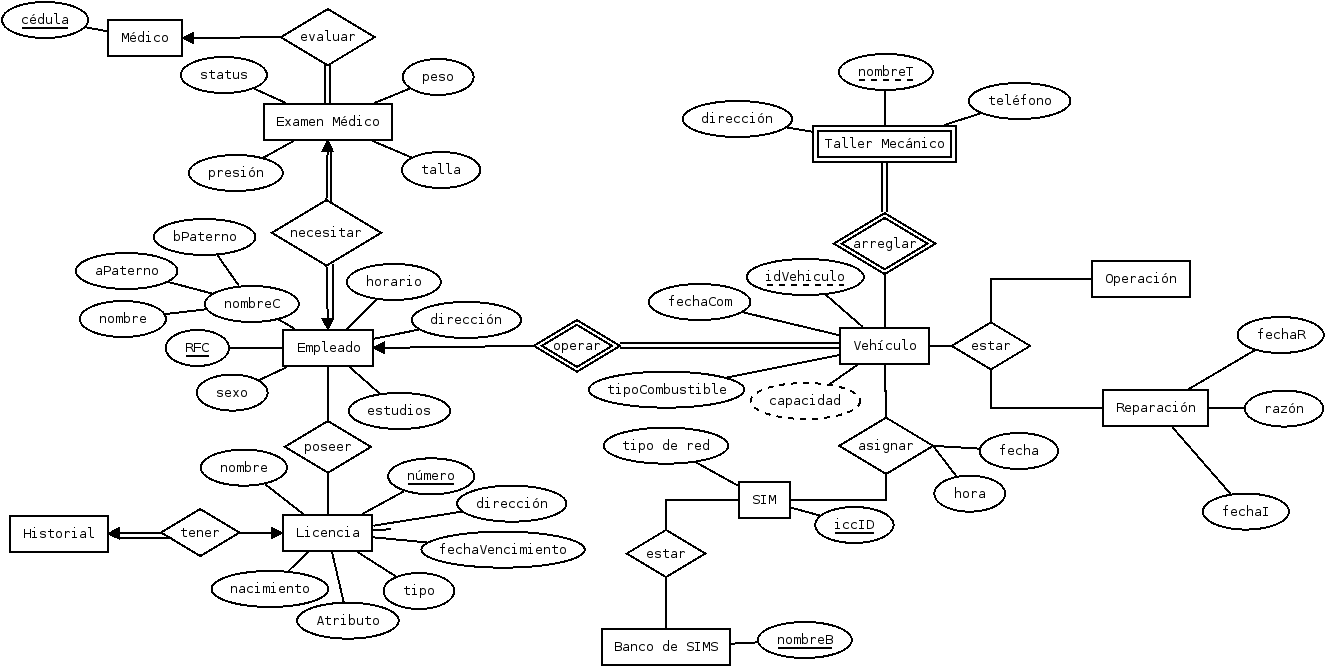
\includegraphics[scale=0.3]{practica3.png}\vspace{.3cm}

        Los cambios realizados para que se modelara el caso de prueba en su
        totalidad se utilizaron los conceptos del modelo entidad-relación 
        extendido como: herencia y agregación.

        Los cambios fueron:

        \begin{itemize}
            \item   Agregamos la entidad "Datos" pues en el modelo anterior en
                    "Empleado" y "Licencia" habían datos repetidos por lo que 
                    colocamos una disyunción total para que dejara de existir
                    redundancia pero el significado no se pierde.
            \item   En al entidad "Vehículo" agregamos un traslape pues en el 
                    modelo anterior se tenía una relación ternaria y así se
                    nota con más claridad lo que se quiere representar.
            \item   También a "Vehículo" agregamos una relación "tener" con 
                    "Ruta" y ésta con una entidad que contiene a "Sitio" y
                    "Estación" para evitar una relación ternaria.
        \end{itemize}

        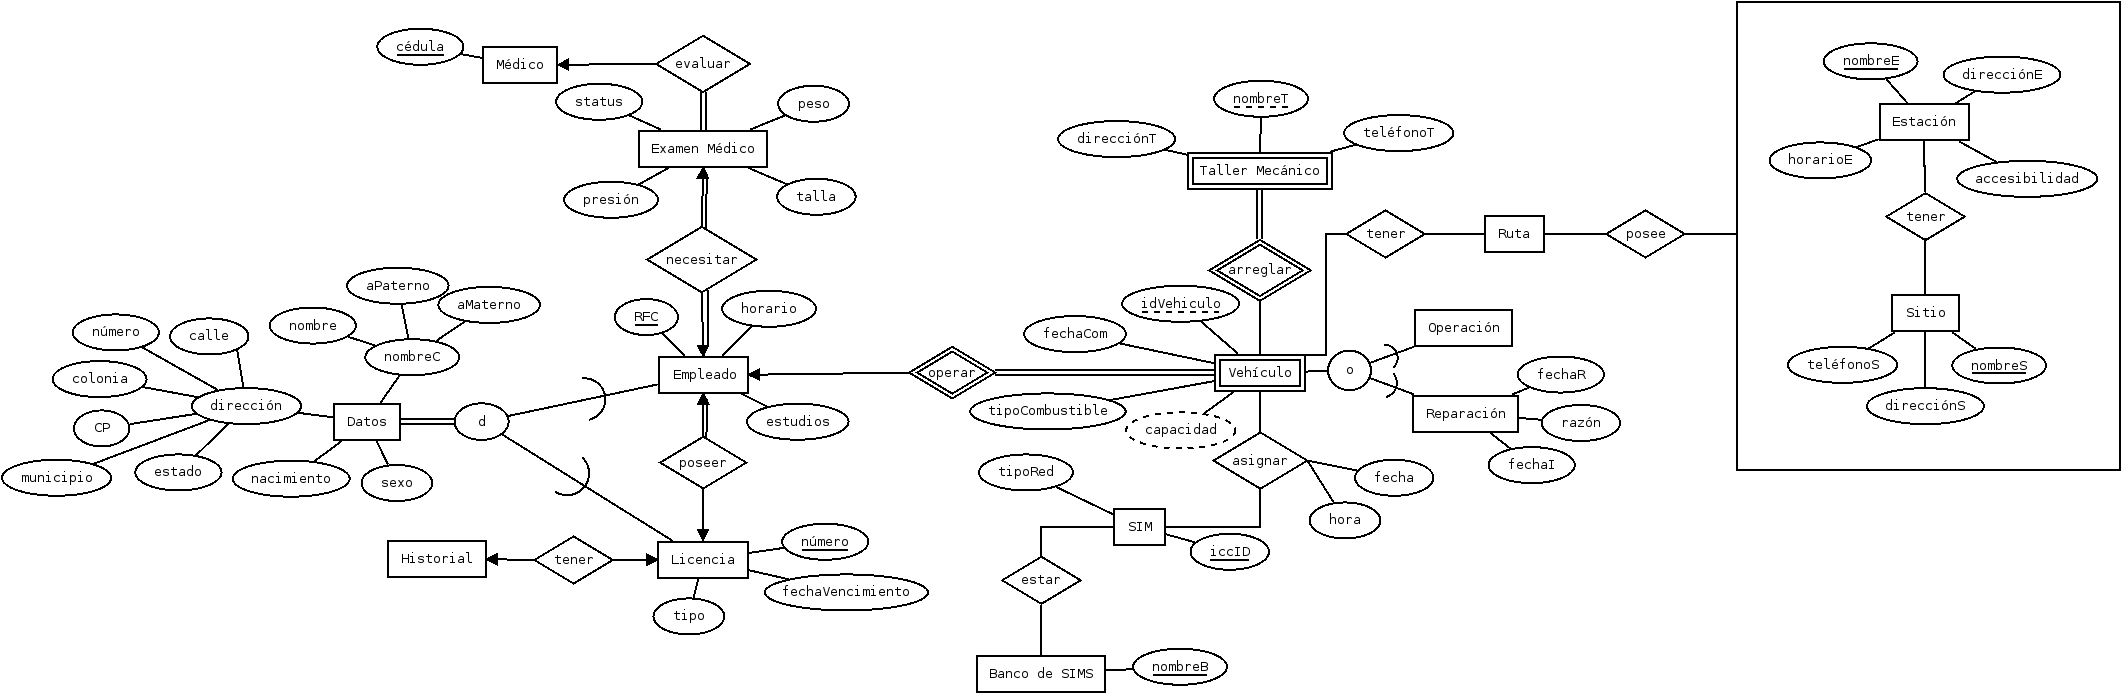
\includegraphics[scale=0.24]{practica4.png}

        \subsection*{Creación de usuario}

        \begin{itemize}
            \item[1.-]  Ejecutamos el siguiente comando para ingresar al contenedor 
                        de docker donde se encuentra SQL-Server. \vspace{.1cm}
             
                \begin{center}
                    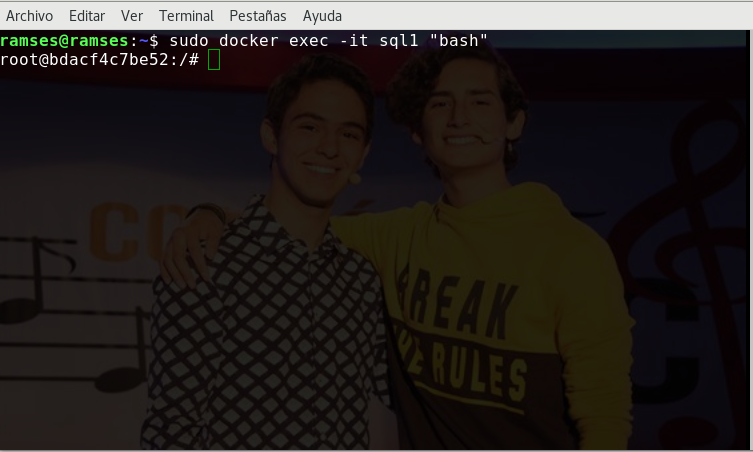
\includegraphics[scale=0.3]{1.png}    
                \end{center}

            \item[2.-]  Dentro del contenedor ingresamos con nuestro usuario (SA) 
                        y la contraseña definida anteriormente; y creamos una 
                        base de datos llamada "lab\_db" con la instrucción
                        CREATE DATABASE. \vspace{.1cm}

                \begin{center}
                    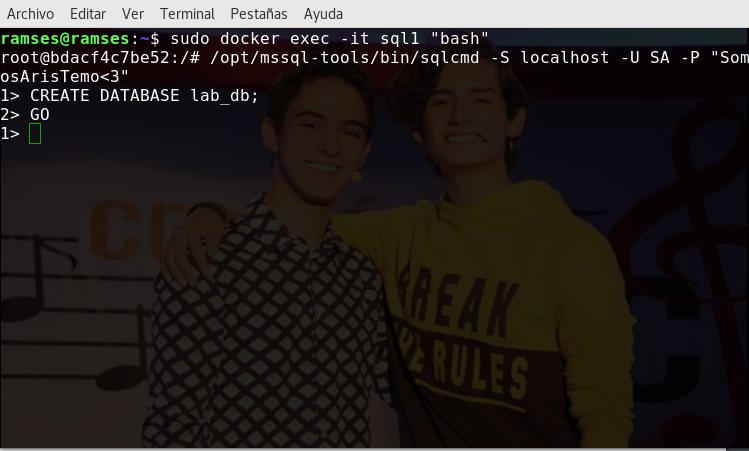
\includegraphics[scale=0.3]{2.png}
                \end{center}

            \item[3.-]  Cambiamos de "master" a "lab\_db" creada en el paso anterior
                        con el comando USE.  \vspace{.1cm}
            
            \begin{center}
                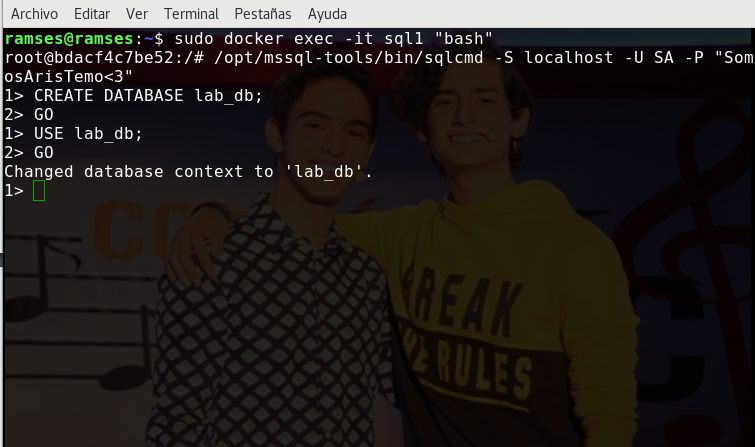
\includegraphics[scale=0.3]{3.png}
            \end{center}

            \item[4.-]  Creamos un login "log\_lab\_p4" con el y una contraseña
            determinada con el comando mostrado a continuación. \vspace{.1cm}
            
            \begin{center}
                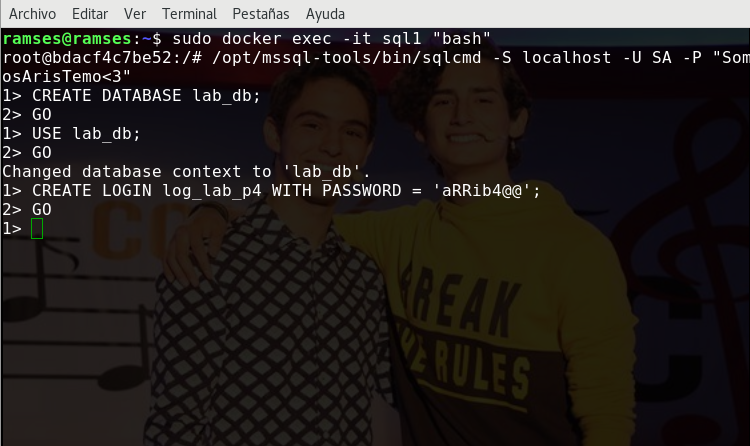
\includegraphics[scale=0.3]{4.png}
            \end{center}

            \item [5.-] Creamos un user "lab\_p4" a definido con el login creado 
                        en el paso anterior. \vspace{.1cm}
            
            \begin{center}
                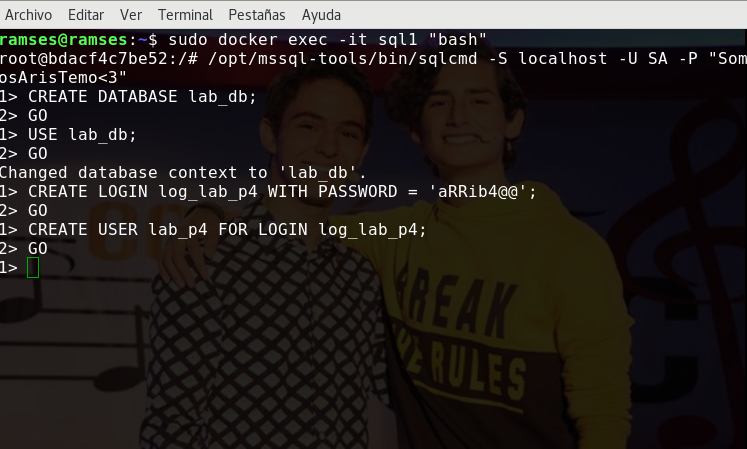
\includegraphics[scale=0.3]{5.png}
            \end{center}

            \item[6.-] Salimos de SQL-SERVER. \vspace{.1cm}
            
            \begin{center}
                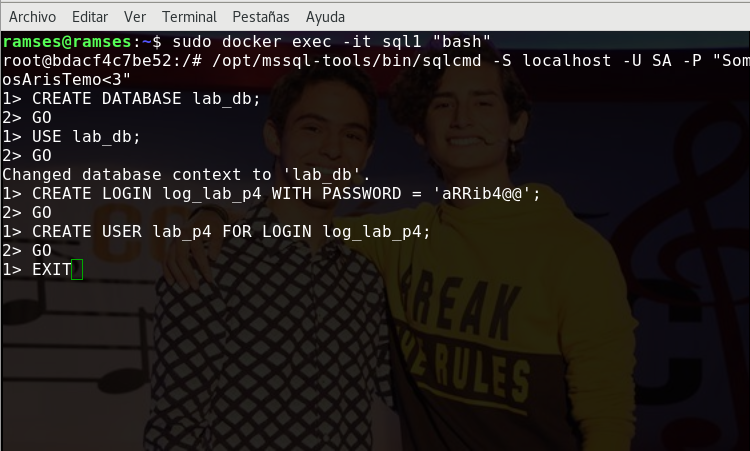
\includegraphics[scale=0.3]{6.png}
            \end{center}

            \item[7.-]  Ingresamos de nuevo a SQL-SERVER con el usuario y contraseña
                        definidos en el paso 4. \vspace{.1cm}
            
            \begin{center}
                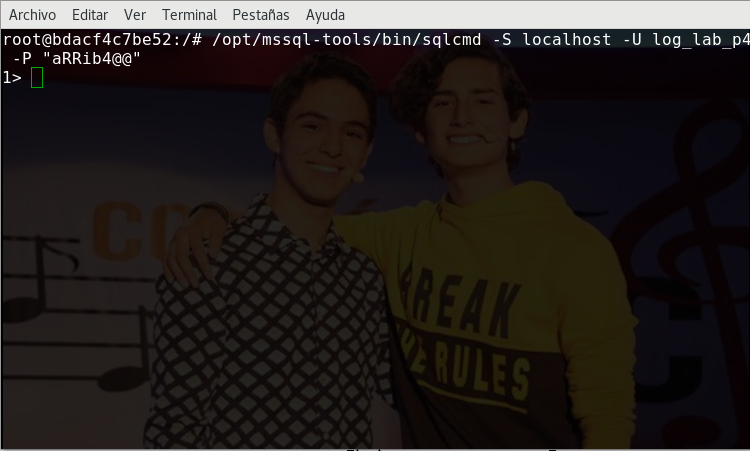
\includegraphics[scale=0.3]{7.png}
            \end{center}

            \item[8.-]  Cambiamos a "lab\_db" para posicionarnos en la base de datos
                        creada en el paso 2.\vspace{.1cm}
            
            \begin{center}
                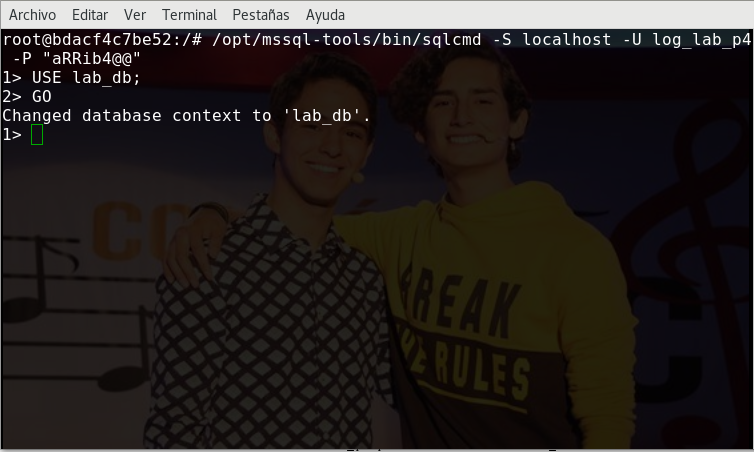
\includegraphics[scale=0.3]{8.png}
            \end{center}

            \item[9.-]  Ejecutamos la siguiente instrucción para visualizar el usuario
                        (por omisión) creado en el paso 5. \vspace{.1cm}
            
            \begin{center}
                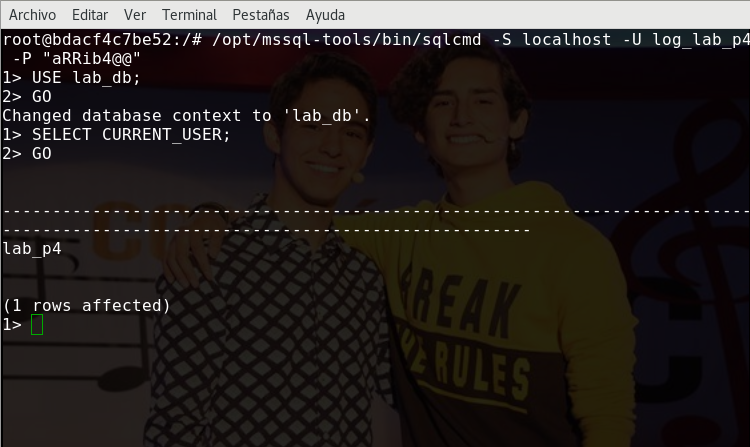
\includegraphics[scale=0.3]{9.png}
            \end{center}

            \item[10.-] Finalmente ejecutamos la instrucción mostrada a continuación para visualizar
                        la base de datos a la cual pertenece el usuario del paso 9. \vspace{.1cm}
            
            \begin{center}
                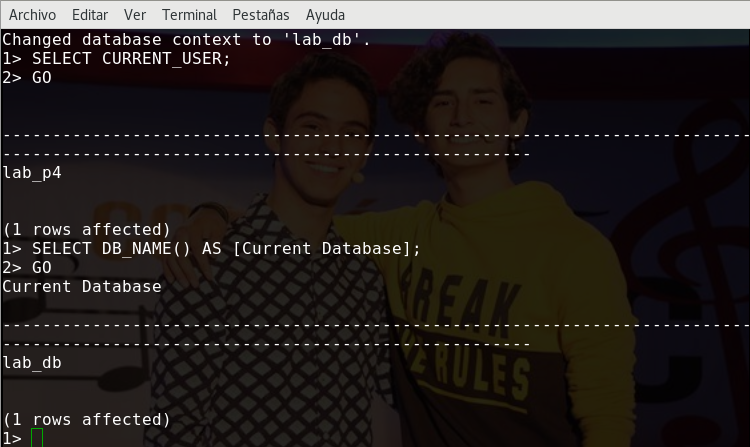
\includegraphics[scale=0.3]{10.png}
            \end{center}

            
        \end{itemize}

    \section*{Conclusión}
    Como se puede notar hicimos uso de los conceptos del modelo entidad-relación extendido.
    Ésta parte de la práctica fue la más sencilla pues al tener el esquema de la práctica
    pasada, sólo eliminamos redundancia y agregamos lo que restaba del caso prueba.\vspace{.3cm}

    En el caso de la creación de usuario nos tomamos más tiempo porque tuvimos problemas con 
    el acceso a contenedor ya definido en prácticas pasadas, por lo que lo tuvimos que 
    reinicializar de nuevo para poder llevar a cabo el procedimiento descrito anteriormente.\vspace{.3cm}

    En conclusión, el modelo entidad-relación extendido nos facilita la manipulación
    de datos que puedan llegar a repetirse en varias entidades y a tener relaciones de grado 
    a lo mas tres. Por otro lado, la creación de un usuario en SQL-Server es necesario tener un 
    login en una base de datos determinada, y con esto podemos tener datos distintos con varios
    logins.

    

\end{document}